    \subsection*{Many Layers}
    
        We are finally ready to build our \textbf{complete} neural network. We'll just retrace the steps of the 2-layer case.\\
        
        \begin{notation}
            The total \purp{number} of \vocab{layers} in our \vocab{neural network} is notated as $L$.
            
            Typically we notate an \purp{arbitrary} layer as $\ell$ (or $l$).
        \end{notation}
        
        Since $x$ is, for all purposes, \textbf{equivalent} to a vector $A$, we will call it $A^0$.\\
        
        \begin{notation}
            Our \vocab{neural network}'s input $x$ is used in the \gren{same} way as every term $A^\ell$.
            
            So, we will \purp{represent} it as 
            
            \begin{equation*}
                x = A^0
            \end{equation*}
        \end{notation}
        
        \begin{figure}[H]
            \centering
            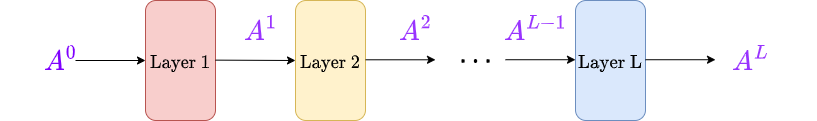
\includegraphics[width=140mm,scale=0.4]{images/nn_images/all_layers.png}
        \end{figure}
        
        Again, we see that the \textbf{output} of layer $\ell$ is the \textbf{input} of layer $\ell+1$.\\
        
        \begin{concept}
            Each layer \vocab{feeds} into the next layer.
            
            $A^\ell$ is the \purp{output} of layer $\ell$, and the \purp{input} of layer $\ell+1$.
            
            This means that the \purp{output} dimension must \gren{match} the next \purp{input} dimension.
            
            \begin{equation*}
                \overbrace{
                    n^\ell
                }^{\text{Output}}
                =
                \overbrace{
                    m^{\ell+1}
                }^{\text{Output}}
            \end{equation*}
            
            And the \vocab{dimension} of $A^\ell$ is $(n^\ell \times 1) = (m^{\ell+1} \times 1)$.
        \end{concept}
        
    \subsection*{Our Complete Neural Network}
    
        We can break our layers into components, so we can see the functions involved. 
        
        With this, we build our final neural network:
        
        \begin{figure}[H]
            \centering
            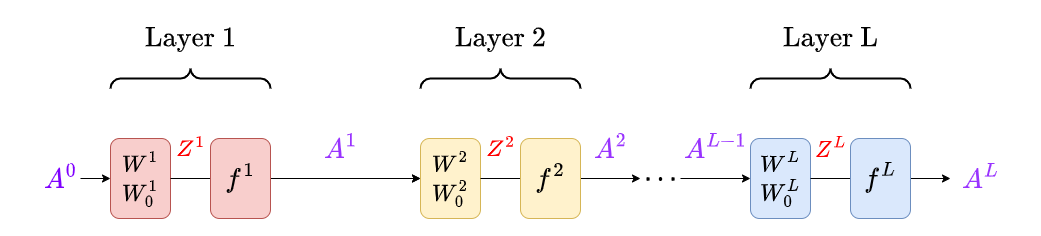
\includegraphics[width=140mm,scale=0.4]{images/nn_images/final_neural_network.png}
        \end{figure}
        
        With this, we can see how each layer is \textbf{related} to each other: as we \textbf{mentioned}, the \textbf{output} of one layer is the \textbf{input} of the next layer.
        
        Here is the computation we do for layer $\ell$:\\
        
        \begin{kequation}
            The calculations done by layer $\ell$ are given by
            
            \begin{equation*}
                \blu{Z^\ell} = (\blu{W^\ell})^T \red{A^{\ell-1}} + \blu{W_0^\ell} 
            \end{equation*}
            
            and
            
            \begin{equation*}
                \blu{A^\ell} = f(\blu{Z^\ell})
            \end{equation*}
            
            Which combine into:
            
            \begin{equation*}
                \blu{A^\ell} = f(\blu{Z^\ell}) = 
                f  
                \Bigg( 
                    (\blu{W^\ell})^T \red{A^{\ell-1}} + \blu{W_0^\ell} 
                \Bigg)
            \end{equation*}
        \end{kequation}

    \subsubsection*{Hidden Layers and the "First Layer"}
        
        Now that we have a full network, we introduce some useful vocab.\\
        
        \begin{definition}
            A \vocab{hidden layer} is any functional layer except for the \purp{output} (last) layer.
            
            It is called a "\gren{hidden}" layer because, if you're viewing the whole neural network based on
            
            \begin{itemize}
                \item \gren{Input} $x$ (first input)
                
                \item \gren{Output} $A^L$ (final output)
            \end{itemize}
            
            You can't see \purp{hidden layers} from outside the network.

            Based on this definition,the \gren{number of hidden layers} in a network is the layer count, minus one: \grn{$L-1$}.
        \end{definition}
        
        Note that there's one point of confusion: online, you may see that the hidden layer is "any layer other than the \textbf{input} (first) or \textbf{output} (last) layer".

        This is because, often, we consider the input itself to be a separate "\textbf{input layer}". 
        
        Despite this fact, when someone counts the number of layers in a neural network, they're usually only counting the hidden and output layers: we \textbf{don't count} the input layer.
            \note{It confused me, too.}\\

        \begin{definition}
            The \vocab{input layer} is a layer that brings the \gren{input} into the network. It applies \purp{no functions} to the data.

            Because the input layer has \purp{no effect} on our data (it just moves it), we \purp{don't count the input layer} when we're saying how \gren{many layers} a network has.
        \end{definition}

        \miniex Consider the following network from earlier:

        \begin{figure}[H]
            \centering
            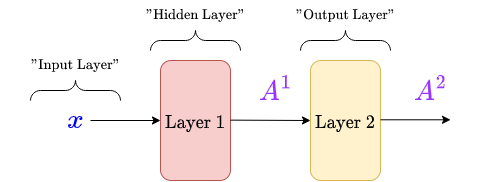
\includegraphics[width=100mm,scale=0.4]{images/nn_images/two_layers_input_layer.png}
        \end{figure}

        In this network, $x$ is passed into the network by the \textbf{input layer}. This layer is \textbf{before} layer 1 (you could think of it as "Layer 0").

        Despite having the input layer, plus layer 1 and 2, we count only
        
        \begin{itemize}
            \item \textbf{Two} layers in our network:
            \begin{itemize}
                \item One hidden layer: Layer 1.
                \item One output layer: Layer 2. 
            \end{itemize}
        \end{itemize}

        